\documentclass[a2paper, 12pt]{article}
\usepackage[font={huge, bf}]{caption}
\usepackage{fontspec}
\setmainfont{Arial}
\usepackage{subcaption}
\usepackage{graphicx}
\usepackage{tikz}
\usepackage{tikzsymbols}
\usetikzlibrary{calc,patterns,shapes.geometric}
\usepackage{float}
\usepackage{pdflscape}
\usepackage{geometry}
\geometry{landscape, margin=2cm}
\captionsetup[subfigure]{justification=justified,singlelinecheck=false}
\pagestyle{empty}

\def\centerarc[#1](#2)(#3:#4:#5){\draw[#1] ($(#2)+({#5*cos(#3)},{#5*sin(#3)})$) arc (#3:#4:#5);}

\begin{document}
	\vspace*{\fill}
	\begin{figure}[!htbp]
		\centering
		\begin{subfigure}[b]{0.48\textwidth}
			\caption{Figure 1}
			\centering
			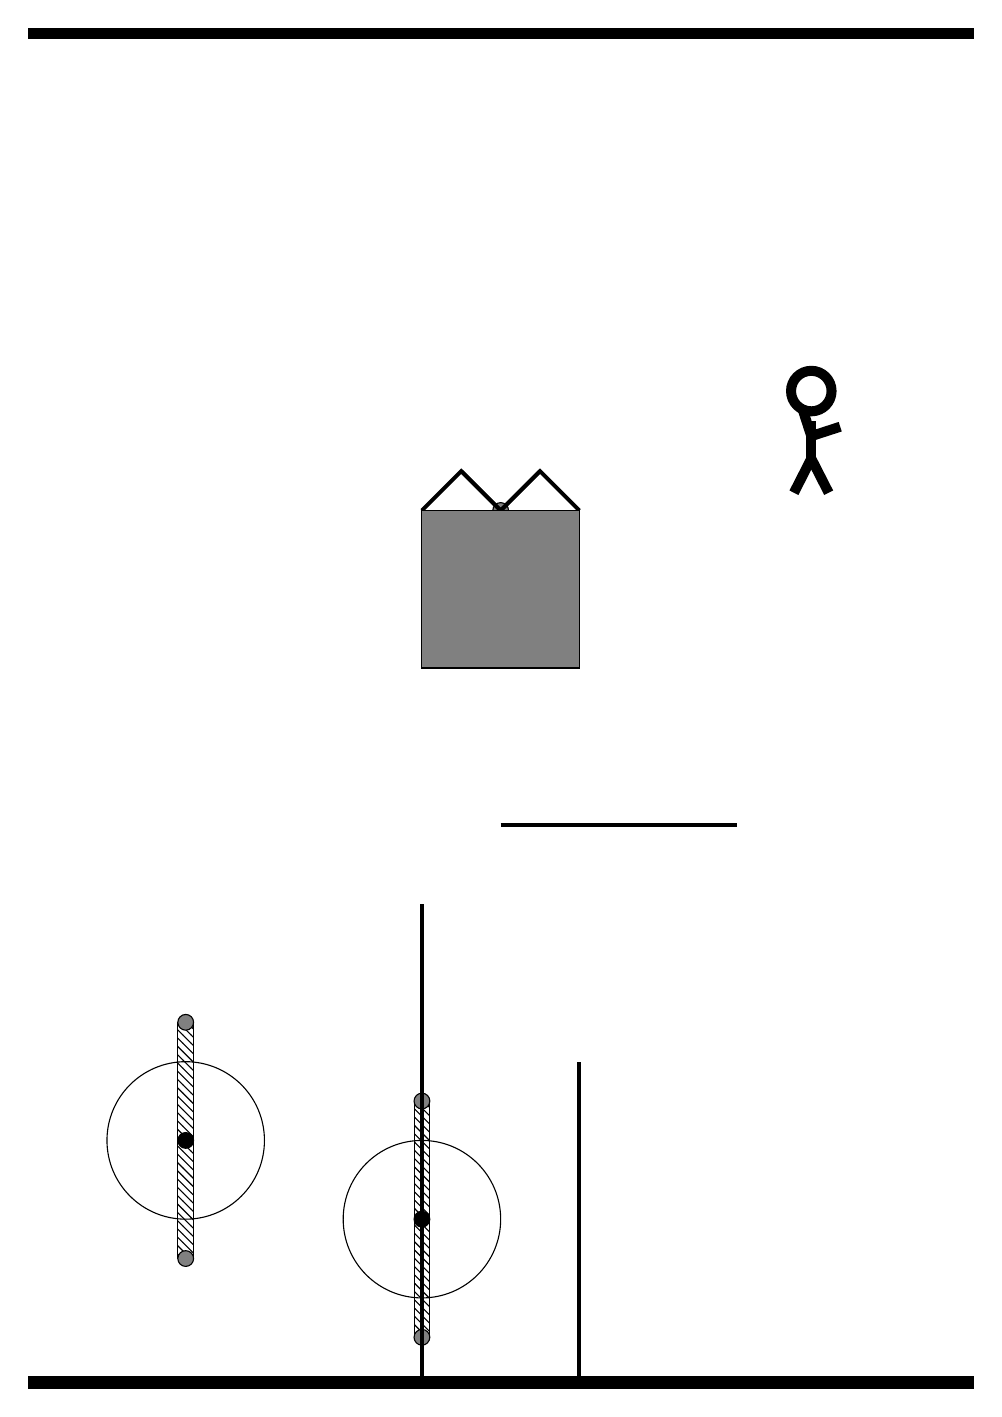
\begin{tikzpicture}
				\draw[fill=black] (-2, 14) rectangle (10, 14.125);
				
				\draw (3,-1) circle (1);
				\draw[fill=black] (3,-1) circle (0.1);
				\draw[pattern=north west lines, pattern color=black] (2.9,0.5) rectangle (3.1,-2.5);
				\draw[fill=black!50] (3,0.5) circle (0.1);
				\draw[fill=black!50] (3,-2.5) circle (0.1);
				
				\draw (0,0) circle (1);
				\draw[fill=black] (0,0) circle (0.1);
				\draw[pattern=north west lines, pattern color=black] (-0.1,1.5) rectangle (0.1,-1.5);
				\draw[fill=black!50] (0,1.5) circle (0.1);
				\draw[fill=black!50] (0,-1.5) circle (0.1);
				
				\draw[fill=black!50] (4,8) circle (0.1);
				\draw[line width=0.5mm](3.5,8.5) -- (4,8) --  (4.5,8.5);
				\draw[line width=0.5mm](3,8) --  (3.5,8.5) -- (4,8) -- (4.5,8.5) -- (5,8);
				\draw[fill=black!50] (3, 8) rectangle (5, 6);
				
				\draw[line width = 0.5mm] (4,4) -- (7,4);
				\centerarc[line width = 0.5mm](4,3)(90:180:1);
				\draw[line width = 0.5mm] (3,3) -- (3,-3);
				\centerarc[line width = 0.5mm](4,-3)(180:360:1);
				\draw[line width = 0.5mm] (5,-3) -- (5,1);
				
				\node at (8, 9) {\scriptsize \Strichmaxerl[10][-162][108]};
				
				\draw[fill=black] (-2, -3) rectangle (10, -3.15);
			\end{tikzpicture}
		\end{subfigure}
		\hfill
		\begin{subfigure}[b]{0.48\textwidth}
			\caption{Figure 2}
			\centering
			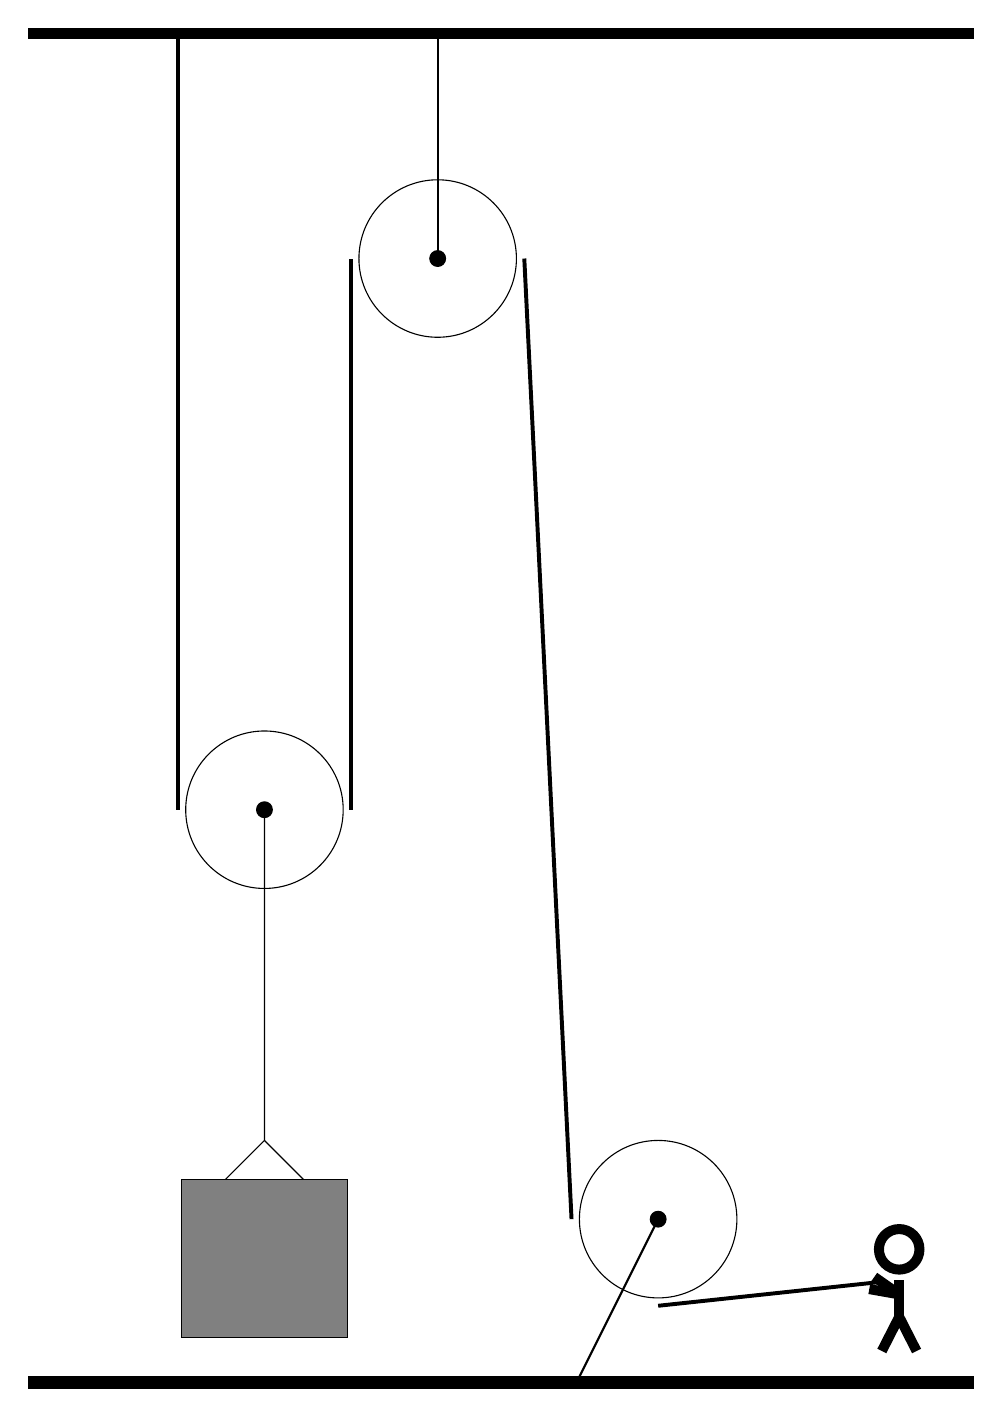
\begin{tikzpicture}
				\draw[fill=black] (-2, 14) rectangle (10, 14.125);
				
				\draw (3.2, 11.2) circle (1);
				\draw[fill=black] (3.2, 11.2) circle (0.1);
				\draw[thick] (3.2, 11.2) -- (3.2, 14);
				
				\draw (6, -1) circle (1);
				\draw[fill=black] (6, -1) circle (0.1);
				\draw[thick] (6, -1) -- (5, -3);
				
				\draw (1, 4.2) circle (1);
				\draw[fill=black] (1, 4.2) circle (0.1);
				
				\draw (1, 4.2) -- (1, 0) -- (0.5, -0.5);
				\draw (1, 0) -- (1.5, -0.5);
				\draw[fill=black!50] (-0.05, -0.5) rectangle (2.05, -2.5);
				
				\draw[line width=0.5mm] (-0.1, 14) -- (-0.1, 4.2);
				\centerarc[line width=0.5mm](1, 4.2)(180:360:1.1);
				\draw[line width=0.5mm](2.1, 4.2) -- (2.1, 11.2);
				\centerarc[line width=0.5mm](3.2, 11.2)(0:180:1.1);
				\draw[line width=0.5mm](4.3, 11.2) -- (4.9, -1);
				\centerarc[line width=0.5mm](6, -1)(180:270:1.1);
				\draw[line width=0.5mm](6, -2.1) -- (8.8, -1.8);
				
				\node at (9, -1.9) {\scriptsize \Strichmaxerl[10][-35][170]};
				
				\draw[fill=black] (-2, -3) rectangle (10, -3.15);
			\end{tikzpicture}
		\end{subfigure}
	\end{figure}
		\vspace*{\fill}
\end{document}